\chapter{Variational inference}
\section{Variational inference}
Variational inference \cite{Bishop_2007,Blei_2017,Murphy_2012,Zhang_2019} is an approximate inference technique that, as Laplace's approximation, tries to approximate a density $g(\theta)$ by some density $q(\theta)$, using the unnormalized density $\gu(\theta) = Z g(\theta)$. In the context of variational inference, this $q(\theta)$ will be called the \textit{variational approximation}. Usually in the context of Bayesian inference, $g(\theta) = p(\theta|\mathcal{D})$ and $\gu(\theta) = p(\mathcal{D}|\theta)p(\theta)$.

Unlike Laplace's approximation, variational inference is concerned in choosing $q(\theta)$ by minimizing a global measure of dissimilarity between the distributions $q(\theta)$ and $g(\theta)$, called a \textit{divergence}. A divergence $D$ on a space $S$ of probability densities with the same support is a function $D(\cdot || \cdot) : S \times S \to \mathbb{R}$ such that:
\begin{equation}
\begin{split}
& D(q||p) \geq 0, \, p,q \in S \\
& D(q||p) = 0 \iff p = q.
\end{split}
\end{equation}
Thus divergences are a weaker form of a distance, and in general most important classes of divergences do not satisfy neither symmetry nor the triangle inequality. The objective of variational inference is then, given the target distribution $g$, and a set of candidate distributions $\mathcal{Q}$, to use a divergence $D$ to find an approximation $q^* \in \mathcal{D}$ for $g$ such that
\begin{equation}\label{viobjective1}
 q^* = \argmin_{q \in \mathcal{Q}} D(q || g).
\end{equation}

If $g \in \mathcal{Q}$, then obviously $q^* = g$. However, $\mathcal{Q}$ is a set of distributions chosen so that its elements are easy to work with, and this is not in general the case for $g$. Usually $\mathcal{Q}$ is parameterized by a set of continuous parameters $\Lambda \subset \mathbb{R}^m$, such that $q(\theta) = q(\theta;\lambda)$. Then, the problem of minimizing \eqref{viobjective1} becomes a continuous optimization problem
\begin{equation}
 \lambda^* = \argmin_{\lambda \in \Lambda} D(q(\cdot;\lambda)||g),
\end{equation}
and $q^*(\theta) = q(\theta;\lambda^*)$

\subsection{KL divergence and evidence lower bound}
Arguably the most important divergence between probability distributions, widely used in information theory, is the \textit{Kullback-Leibner} (KL) divergence $D_{KL}$, given by \footnote{The KL divergence has origins in information theory, and for discrete distributions, it can be interpreted as the average additional information one has to transmit a receiver when you are modeling a random variable distributed according to $q$ by $p$ \cite{Murphy_2012}}
\begin{equation}
D_{KL}(q||p) = -\Ev_{\theta \sim q(\theta)} \left[ \log \frac{p(\theta)}{q(\theta)} \right].
\end{equation}
Variational inference has in general the minimization objective $D_{KL}(q||g)$, although some recent methods have been concerned with other divergence objectives  \cite{Hernandes-Lobato_2015,Yingzhen_2016,Wang_2018} \footnote{Some authors reserve the term variational inference just for the objective $D_{KL}(q||g)$}. Notice that, since $D_{KL}(q||g) \neq D_{KL}(g||q)$, minimizing $D_{KL}(q||g)$ is different from minimizing $D_{KL}(g||q)$. In fact, the later minimization objective ends up with the related \textit{expectation propagation} technique for approximate inference \cite{Bishop_2007}. In this work we are mainly concerned with the variational inference $D_{KL}(q||g)$ objective.

Since $g(\theta) = \gu(\theta)/Z$, $D_{KL}(q||g)$ can be rewritten as:
\begin{equation}
D_{KL}(q||g) = -\bigg(\Ev_{\theta \sim q(\theta)}[\log \gu(\theta)] -\Ev_{\theta \sim q(\theta)}[\log q(\theta)]\bigg) + \log Z,
\end{equation}
The quantity inside parenthesis is called the \textit{evidence lower bound} (ELBO)
\begin{equation}\label{elbodef}
\mathcal{L}_\gu(q) = \Ev_{\theta \sim q(\theta)}[\log \gu(\theta)] + \mathcal{H}(q),
\end{equation}
where $\mathcal{H}(q) := -\Ev_{\theta \sim q(\theta)}[\log(q(\theta))]$ is the differential entropy of $q$.

In general, the dependence on $\gu$ will be omitted until Section \ref{vbmc_section}, and the ELBO will be denoted as $\mathcal{L}(q)$. Minimizing $D_{KL}(q||g)$ is equivalent to maximizing $\mathcal{L}(q)$. This way, there is no need to calculate the normalization factor $Z$, thus markedly improving the flexibility of the method, and the goal becomes
\begin{equation}
q^* = \argmax_{q \in \mathcal{Q}} \mathcal{L}(q).
\end{equation}
The ELBO is so called because, considering again $p(\theta|\mathcal{D})$, we have that 
\begin{equation}
\begin{split}
\log p(\mathcal{D}) & = \log \Ev_{\theta \sim p(\theta)} [p(\mathcal{D}|\theta)] \\
& = \log \Ev_{\theta \sim q(\theta)} \left[\frac{p(\mathcal{D}|\theta) p(\theta)}{q(\theta)} \right] \\
& \geq \Ev_{\theta \sim q(\theta)} \left[ \log \frac{p(\mathcal{D}|\theta) p(\theta)}{q(\theta)} \right] = \mathcal{L}(q).
\end{split}
\end{equation}
So the ELBO provides a lower bound for the evidence of the model. This means that, when doing model selection between various models $M_1$,\ldots,$M_t$, one can find their corresponding variational distributions $q^*_{M_1},\ldots,q^*_{M_t}$ and $\mathcal{L}(q^*_{M_t}),\ldots,\mathcal{L}(q^*_{M_t})$, and then choose the model $M$ with the maximum $\mathcal{L}(q^*_{M})$, as a proxy for \eqref{modelselectionobjective}. Notice that this is a heuristic, and there is no guarantee that the model with maximum ELBO is actually the one with maximum evidence.

\subsubsection{Qualitative interpretations}
One possible interpretation for maximizing the ELBO is that maximizing the first ELBO term 
\begin{equation}\label{elboterm1}
 \Ev_{\theta \sim q(\theta)}[\log \gu(\theta)],
\end{equation}
is the algorithm \enquote{trying} to make $q$ have a high probability density wherever $\gu$ has a high unnormalized density, while maximizing the second ELBO term,
\begin{equation}
 \mathcal{H}(q) = -\Ev_{\theta \sim q(\theta)}[\log q(\theta)],
\end{equation}
acts as a sort of regularizer preventing $q$ to degenerate to a point mass at the maximum of $\gu$.

It is informative to understand qualitatively which kind of approximations of $g$ variational inference will seek. Suppose some algorithm minimizes $D_{KL}(q || g)$ for $q \in \mathcal{Q}$. Since the algorithm \enquote{wants} to make the integrand $q(\theta) (\log q(\theta) - \log g(\theta))$ small, where $g(\theta)$ is close to zero, the $-\log g(\theta)$ term will quickly become large, unless $q(\theta)$ is also close to zero there. However, where $g(\theta)$ is reasonable far away from zero, the algorithm will not \enquote{feel} as much pressure to match $q(\theta)$ to the same value, provided that the algorithm assign large values for $q(\theta)$ where $g(\theta)$ is already large. Then, variational inference will tend to underestimate the region where $g(\theta)$ is large. By contrast, expectation propagation will have the reverse behavior, overestimating the region where $g(\theta)$ is far from zero \cite{Bishop_2007}. This is shown in Figure \ref{vixepfigure}.

\begin{figure}
	\centering
	\subfloat[$D_{KL}(q||g)$ ]{\label{vixep1a}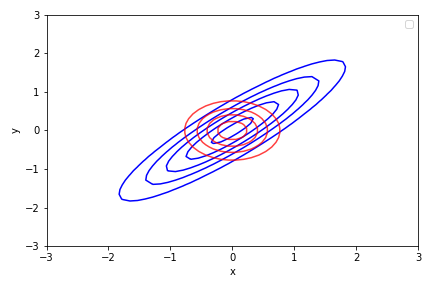
\includegraphics[width=0.3\textwidth]
		{figs/klil3a.png}}
	\subfloat[$D_{KL}(g||q)$]{\label{vixep1b}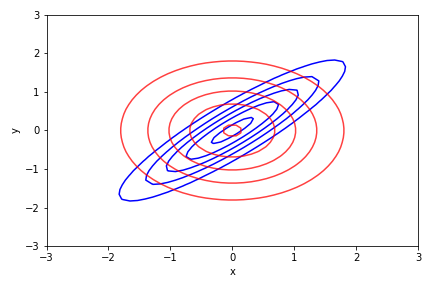
\includegraphics[width=0.3\textwidth]
		{figs/klil3b.png}}


	\caption[Difference of behavior when minimizing $D_{KL}(q||g)$ and $D_{KL}(g||q)$]{\label{vixepfigure} Difference of behavior when minimizing $D_{KL}(q||g)$ (a) and when minimizing $D_{KL}(g||q)$ (b). Here the true distribution (in blue) is approximated by a multivariate normal distribution with diagonal covariance (in red). Example inspired by \cite{Bishop_2007}. Generating code can be found in \url{https://github.com/DFNaiff/Dissertation/blob/master/illustrations_dissertation/kl_illustrative_2.py}.}
\end{figure}

\section{Mean field variational inference}
Traditionally, variational inference has mainly been concerned with factorized variational approximations of the form $q(\theta;\lambda) = \prod_{i=1}^D q_i(\theta_i;\lambda_i)$, called \textit{mean field approximation}. The use of such variational posterior greatly simplifies the optimization of ELBO by coordinate descent. 

To see this, consider a single term $j$ of the variational approximation $q(\theta) = \prod_{i=1}^D q_i(\theta)$. The ELBO for $q(\theta)$ is:
\begin{equation} \label{mfviexpansion}
\begin{split}
\mathcal{L}(q) & = \int \log \gu(\theta) \prod_{i=1}^D q_i(\theta_i) d \theta - \int \left(\sum_{j=1}^D \log q_i(\theta_i) \right) \prod_{i=1}^D q_i(\theta_i) d \theta \\
	     & = \int q_j(\theta_j) \left( \int \log \gu(\theta) \prod_{i \neq j} q_i(\theta_i) d \theta_i \right) d\theta_j + \sum_{i=1}^D \mathcal{H}(q_i) \\
	     & = \int q_j(\theta_j) \log \phi_j (\theta_j) d\theta_j + \mathcal{H}(q_j) + \sum_{i\neq j} \mathcal{H}(q_i),
\end{split}
\end{equation}
With
\begin{displaymath}
\log \phi_j(\theta_j) := \int \log(\gu(\theta)) q_{-j}(\theta_{-j}) d\theta_{-j} = \Ev_{\theta_{-j} \sim q_{-j}} [ \log \gu(\theta) ],
\end{displaymath}
using the notation $q_{-j}(\theta_{-j}) = \prod_{i\neq j}q_i(\theta_i)$.
Now, assuming $\exp ( \log \phi_j(\theta_j))$ to be integrable over the support of $g(\theta)$, fix every $q_i$ for $i \neq j$, so that the only term to be maximized is $q_j$. Then, maximizing \eqref{mfviexpansion} in respect to $q_j$ is equivalent to maximizing the ELBO between $q_j$ and $\exp \left(\log \phi_j(\theta_j)\right) $. Since there are not any constraints in the choice for $q_j$
\begin{equation} \label{mfviqj}
q^{*}_j(\theta_j;q_{-j}) \propto \exp \Ev_{\theta_{-j} \sim q_{-j}} [ \log \gu(\theta)].
\end{equation}
This readily gives an algorithm to find $q^* = \prod q^*_j$: initialize $q_1,\ldots,q_D$ in a appropriate manner, and then optimize cyclically \eqref{mfviqj}. 

Convergence is guaranteed due to the convexity of the bound with respect to each factor \cite{Bishop_2007,Boyd_2004}. This algorithm interacts well with target densities whose conditional distributions $g(\theta_j|\theta_{-j})$ belongs to the exponential family, that is, 
\begin{equation}\label{exponential_family}
 g(\theta_j|\theta_{-j}) = h(\theta_j) \exp \left( \eta_j(\theta_{-j})^T t(\theta_j) - a(\eta_j(\theta_{-j})) \right),
\end{equation}
\eqref{mfviqj} reduces to \cite{Blei_2017} 
\begin{equation}
 q^*_j(\theta_j;q_{-j}) \propto h(\theta_j) \exp \left( \Ev_{\theta_j \sim q_{-j}} [\eta_j(\theta_{-j})]^T t(\theta_{-j}) \right),
\end{equation}
thus if $\nu_j = \Ev_{\theta_{-j} \sim q_{-j}}[\eta_j(\theta_{-j})]^T$ is available analytically, the coordinate descent becomes relatively simple.

Research to extend mean field variational inference to large datasets or dimensionality exists \cite{Hensman_2012,Hoffman_2013,Zhang_2019}, however factorized limitations are limited, particularly in its independence assumption. Moreover, many distributions are not in the exponential family, which is the focus of the mean field method, so more generic methods are desirable.

\section{Generic variational inference}
Some recent advances in variational inference \cite{Zhang_2019} are concerned with expanding both the set of possible variational approximations $\mathcal{Q}$ and approximating general classes of posterior distributions $g(\theta)$. 

Considering again $\mathcal{Q}$ to be parameterized by a continuous set of parameters $\Lambda$, and using the overloaded notation $\mathcal{L}(\lambda) = \mathcal{L}(q(\cdot;\lambda))$, return to the optimization problem 
\begin{equation}
\begin{split}
\lambda^* = \argmax_{\lambda \in \Lambda} \mathcal{L}(\lambda) & = \argmax_{\lambda \in \Lambda} \left( \Ev_{\theta \sim q(\theta;\lambda)}[\log \gu(\theta)] + \mathcal{H}(q(\cdot;\lambda)) \right)\\
& =  \argmax_{\lambda \in \Lambda} \Ev_{\theta \sim q(\theta;\lambda)}\left[\log \left(\frac{\gu(\theta)}{q(\theta;\lambda)}\right)\right]
\end{split}
\end{equation}
In general the expectations involved cannot be calculated analytically. However, if one represents $\nabla \mathcal{L}(\lambda)$ as expectations, then by using Monte Carlo methods it is possible to use stochastic gradients methods \cite{Robbins_1951,Kingma_2014,Qian_1999,Ruder_2016} to maximize $\mathcal{L}(\lambda)$ \footnote{In this aspect, modern variational inference research benefits greatly from deep learning research, the later relying heavily on stochastic gradient descent, driving much of the recent development of these algorithms.}.

\subsection{REINFORCE}
One proposal for doing this is given in \cite{Wingate_2013} and \cite{Ranganath_2014}, where $\nabla \mathcal{L}(\lambda)$ is rewritten as \footnote{A quick derivation of this approximation is done in the Appendix \ref{appendixreinforce}.}
\begin{equation}\label{reinforce}
\nabla \mathcal{L}(\lambda) = \Ev_{\theta \sim q(\theta;\lambda)} \left[ \log \frac{\gu(\theta)}{q(\theta;\lambda)} \nabla_{\lambda} \log q(\theta;\lambda) \right], 
\end{equation}
and is approximated with its Monte Carlo estimator 
\begin{equation}\label{reinforcemc}
\nabla \mathcal{L}(\lambda) \approx \frac{1}{K} \sum_{i \in [K], \theta_i \sim q(\theta;\lambda)} \log \frac{\gu(\theta_i)}{q(\theta_i;\lambda)} \nabla_{\lambda} \log q(\theta_i;\lambda),
\end{equation}
where $[K] = \{1,\ldots,K\}$. In practice, this estimation suffers from high variance, which may hinder optimization. In \cite{Wingate_2013}, \eqref{reinforce} is substituted for 
\begin{equation}
\nabla \mathcal{L}(\lambda) = \Ev_{\theta \sim q(\theta;\lambda)} \left[ \left( \log \left( \frac{\gu(\theta)}{q(\theta;\lambda)}\right) + C\right) \nabla_{\lambda} \log q(\theta;\lambda) \right], 
\end{equation}
where $C$ is an arbitrary constant, which is adjusted to control variance \footnote{The reason that this constant can be added is because $\int C \nabla_\lambda \log q(\theta;\lambda) q(\theta;\lambda) d\theta = C \int \nabla_\lambda p(\theta;\lambda) d\theta = C \nabla_\lambda \int p(\theta;\lambda) d\theta = 0$.}. In \cite{Ranganath_2014}, the variance is controlled by Rao-Blackwellization and control variates instead. Other variance reduction methods for this gradient formulation are proposed in \cite{Titsias_2015} and \cite{Ruiz_2016}.

\subsection{Reparameterization trick}\label{reparameterizationsection}
An alternative to calculate the gradient of $\mathcal{L}(\lambda)$ as an expectation is known as the \textit{reparameterization trick} \cite{Kingma_2013}, which is a general technique for calculating gradients of expectations of continuous random variables.

To explain the general ideia, assume $X_\lambda$ is a continuous random variable distributed according to $f(x;\lambda)$, and one wants to calculate the gradient (in relation to $\lambda$) of
\begin{equation}\label{reparamderiv1}
\Ev_{X_\lambda} \left[ h(X_\lambda) \right] = \int h(x) f(x;\lambda) dx.
\end{equation}
We approximate \eqref{reparamderiv1} by Monte Carlo
\begin{equation}\label{reparamderiv2}
\Ev_{X_\lambda} \left[ h(X_\lambda) \right] \approx \sum_{i=1}^N h(x_{i,\lambda}), \quad x_{i,\lambda} \sim f(x;\lambda).
\end{equation}
Now suppose that there is some random variable $Y$, \textit{not depending on $\lambda$}, with density $r(y)$, such that $X_\lambda = s(Y;\lambda)$ (for instance, if $X_{\mu,\sigma} \sim \mathcal{N}(\mu,\sigma^2)$, then being $Y \sim \mathcal{N}(0,1)$, we have that $X_{\mu,\sigma} = s(Y;\mu,\sigma) = \sigma Y + \mu$). In this case, the Monte Carlo estimator \eqref{reparamderiv2} is rewritten as
\begin{equation}
\Ev_{X_\lambda} \left[ h(X_\lambda) \right] \approx \sum_{i=1}^N h(s(y_i,\lambda)), \quad y_i \sim r(y),
\end{equation}
which is an expression \textit{whose gradient in relation to $\lambda$ can be taken}, and is the Monte Carlo estimator of
\begin{equation}
\int h(s(y;\lambda)) r(y) dy = \Ev_Y [h(s(Y;\lambda))]
\end{equation}

Formally, by letting $A$ be the support of $Y$ and $B_\lambda$ be the support of $X_\lambda$, if $s(y;\lambda)$ if bijective with injective derivative:
\begin{equation}
\begin{split}
\Ev_{X_\lambda \sim f(x;\lambda)} [h(x)] & = \int_{B_\lambda} h(x) q(x;\lambda) dx \\
& = \int_A h(s(y;\lambda)) q(s(y;\lambda);\lambda) |\text{det} (s'(y;\lambda))| dy \\
& = \int_A h(s(y;\lambda)) r(y) dy = \Ev_{Y \sim r(y)} [h(s(y;\lambda))],
\end{split}
\end{equation}
which shows that the reparameterization trick is valid.

To apply this to $\mathcal{L}(\lambda)$, assume $\theta_\lambda \sim q(\theta;\lambda)$ is such that $\theta_\lambda = s(\epsilon;\lambda)$, with $\epsilon \sim r(\epsilon)$. Then, applying reparameterization, we have
\begin{equation}\label{mcreparameterization}
\begin{split}
 \nabla \mathcal{L}(\lambda) & = \nabla \left(\Ev_{\theta \sim  q(\theta;\lambda)}\left[\log \frac{\gu(\theta)}{q(\theta;\lambda)}\right] \right) \\
 & =\nabla \left( \Ev_{\epsilon \sim r(\epsilon)} \left[\log \frac{ \gu(s(\epsilon;\lambda))}{q(s(\epsilon;\lambda);\lambda)}\right]\right) \\
 & \approx \nabla_\lambda \left( \frac{1}{K} \sum_{i \in [K], \epsilon_i \sim r(\epsilon)} \log \frac{ \gu(s(\epsilon_i;\lambda))}{q(s(\epsilon_i;\lambda);\lambda)} \right)
\end{split}
\end{equation}
In \cite{Zhang_2019}, it is argued that the observed lower variance of this estimation methods, if compared to the one given by \eqref{reinforce}, may be due to the fact that reparameterization trick takes in account the gradient of the target distribution, instead of just the gradient of the variational distribution as in \eqref{reinforce}. Moreover, in cases that the entropy of $q(\cdot;\lambda)$ can be estimated analytically, the reparameterization trick can be applied only to $\gu(\theta)$, leading to lower variance. Finally, it is important to notice that this format is more readily integrated in an automatic differentiation package, since it suffices to calculate the sum inside the gradient and backpropagate it in relation to $\lambda$.

\iffalse
These recent advances in the field, allowing the application of variational inference for a general variety of target distributions, has resulted in the technique return to some popularity, with recent probabilistic programming language focusing on it, such as Pyro \cite{Bingham_2018} and Edward \cite{Tran_2016}.
\fi

\section{Mixtures of gaussians for variational approximations}\label{mixgaussiansvi}

The idea of using mixture distributions for variational inference dates back to the late 90s \cite{Bishop_1997,Jaakkola_1998}, originally developed for a limited number of target distributions, and later is explored for approximating general distributions in \cite{Gershman_2012,Salimans_2012}, leading to recent work in it \cite{Acerbi_2018,Arenz_2018,Guo_2016,Jankowiak_2019,Miller_2016}. The technique presented here uses the reparameterization trick, in a vein similar to the one presented in \cite{Miller_2016}. In general, the mixture distribution considered is one of Gaussian distributions (as it is in this work), although many of those extends to more general mixtures.

More formally, consider as the set of candidate proposals 
\begin{equation}
\mathcal{Q}_k := \left\{\sum_{i=1}^k w_i f(\cdot;\lambda_i) \middle| f(\cdot;\lambda_i) \in \mathcal{Q}_1, 1 \leq i \leq k; (w_1,...,w_k) \in \Delta_k \subset \mathbb{R}^k \right\},
\end{equation}
wher $\Delta_k$ denotes the probability simplex $\{(x_1,\ldots,x_k) \in {\mathbb{R}^+}^k| \sum_{i=1}^k x_k = 1\}$, and $\mathcal{Q}_1 = \{f(\cdot;\lambda) | \lambda \in \Lambda \subset \mathbb{R}^m\}$ is a parameterized set of distributions. In the mixture of multivariate normals case,
\begin{equation}
\mathcal{Q}_1 := \{f(\cdot ; \mu,\Sigma) = \mathcal{N}(\cdot;\mu,\Sigma) | \mu \in \mathbb{R}^d,\Sigma \in \mathbb{R}^{d \times d}, \Sigma \geq 0\} 
\end{equation}
is the set of multivariate normal distributions. In many cases, it is interesting to restrict $\mathcal{Q}_1$ further so that $\Sigma$ is diagonal.
Mixtures of distributions are interesting as variational approximations since their expectations are easily available 
\begin{equation}
\Ev_{X \sim \sum_i w_i f_i} [h(X)] = \sum_i w_i \Ev_{X_i \sim f_i} [h(X_i)],
\end{equation}
as well as their covariances
\begin{equation}
\begin{split}
& \Cov_{X \sim \sum_i w_i f_i}(X) = \sum_i w_i \left( \Sigma_i +   \mu_i \mu_i^T \right) - \mu \mu^T, \\
& \Sigma_i = \Cov_{X_i \sim f_i}(X_i), \quad \mu_i = \Ev_{X_i \sim f_i}[X], \quad \mu = \Ev_{X \sim \sum_i w_i f_i} [X].
\end{split}
\end{equation}
Furthermore, samples of mixtures can be easily generated from the base distributions, by choosing mixture $i$ with probability $w_i$, and then sampling $X$ from $f(\cdot;\lambda_i)$ \footnote{Batching this process in order to sample many variables, escaping loops in interpreted languages with support for numerical operations (such as Python with Numpy) requires some care, but it is possible in few lines.}. Furthermore, letting $\mathcal{Q}_\infty = \cup_{i=1}^\infty \mathcal{Q}_i$ and $\mathcal{Q}_1$ be these set of Gaussian distributions, $\mathcal{Q}_\infty$ is dense in the set of continuous distributions \cite{Epanechnikov_1969}, so in this case any continuous distribution can be approximated arbitrarily close, in principle.

Considering mixtures of Gaussians, for fixed $k$, in order to find the parameters
\begin{displaymath} 
\lambda = (w_1,\mu_1,\Sigma_1,\ldots,w_k,\mu_k,\Sigma_k)
\end{displaymath}
of 
\begin{equation}
 q^*_k = \argmax_{q_k \in \mathcal{Q}_k} \mathcal{L}(q_k),
\end{equation}
one needs first to find suitable parameterizations for $\Sigma_i$ and $\mathbf{w} := (w_1,...,w_k)$. For the covariance matrix, one can either consider only diagonal matrices
\begin{equation}
\Sigma_i = \text{diag}(\sigma^2_{i,1},\ldots,\sigma^2_{i,D}),
\end{equation}
or consider matrices of the form
\begin{displaymath}
 \Sigma_i = \u_i \u_i^T + \text{diag}(\sigma^2_{i,1},\ldots,\sigma^2_{i,D}),
\end{displaymath}
or use more advanced parameterizations such as the ones found in \cite{Pinheiro_1996}. Let $\sigma_i$ be the parameters for $\Sigma_i$, so that $\Sigma_i = \Sigma_i(\sigma_i)$. For $\mathbf{w}$, using some monotone bijective differentiable function $\phi : \mathbb{R} \to \mathbb{R}^+$ (for example, $\phi = \exp$), one can then consider the corresponding differentiable map $\Phi : \mathbb{R}^k \to \Delta_k$ as 
\begin{equation}
\Phi(\nu_i) = \frac{\phi(\nu_i)}{\sum_{i=1}^k \phi(\nu_k)} = w_i(\nu_i).
\end{equation}

The parameter of interest $\lambda$ becomes $(\nu_1,\mu_1,\sigma_1,\ldots,\nu_k,\mu_k,\sigma_k)$, and
\begin{equation}
q_k(\theta) = \sum_{i=1}^k w_i(\nu_i) f_{\mathcal{N}(\mu_i,\Sigma(\sigma_i))}(\theta).
\end{equation}
Thus, the ELBO objective becomes
\begin{equation}\label{elbomixturegaussians}
\begin{split}
\mathcal{L}(\lambda) & = \int \log \gu(\theta) q_k(\theta) d\theta - \int \log (q_k(\theta)) q_k(\theta) d \theta \\
& = \sum_{i=1}^k w_i(\nu_i) \Ev_{\theta_i \sim \mathcal{N}(\mu_i;\Sigma(\sigma_i))}\left[\log \frac{ \gu(\theta_i)}{q_k(\theta_i;\lambda)}\right].
\end{split}
\end{equation}

One can adapt the reparameterization trick to rewrite $\mathcal{L}(\lambda)$ in a manner suitable to stochastic gradient optimization. First notice that any gaussian random variable $X \sim \mathcal{N}(\mu,\Sigma)$ can be written as $X = \mu + A Z$, where $Z \sim \mathcal{N}(0,I)$ and $A$ is some matrix such that $\Sigma = A A^T$. For instance, $A$ can be the lower Cholesky factor of $\Sigma$, if the parameterization of $\Sigma$ only supports positive-definite matrices. Then $A(\sigma)$ is differentiable \cite{Smith_1995,Murray_2016}, and $s(\epsilon;\mu_i,\sigma_i) = \mu_i + A(\sigma) \epsilon$, and \eqref{elbomixturegaussians} is approximated by Monte Carlo,
\begin{equation}\label{mcmixturegaussians}
\begin{split}
\mathcal{L}(\lambda) & = \sum_{i=1}^k w_i(\nu_i) \Ev_{\epsilon \sim \mathcal{N}(0,I)}\left[\log \frac{ \gu(s(\epsilon;\mu_i,\sigma_i))}{q_k(s(\epsilon;\mu_i,\sigma_i);\lambda)}\right] \\
& \approx \sum_{i=1}^k w_i(\nu_i) \left( \frac{1}{K_i} \sum_{k \in [K_i], \epsilon_{i,j} \sim \mathcal{N}(0,I)} \log \frac{ \gu(s(\epsilon_{i,j};\mu_i,\sigma_i))}{q_k(s(\epsilon_{i,j};\mu_i,\sigma_i);\lambda)} \right),
\end{split}
\end{equation}
which is an expression that can be differentiated to find an approximation for $\nabla \mathcal{L}(\lambda)$.

In principle there is no way to know how many mixtures are necessary to return a good approximation. However, one can,for each $i \in \mathbb{N}$, starting with $i = 1$, sequentially find $q^*_i$ close to $\argmax_{q_i \in \mathcal{Q}_i} \mathcal{L}(q)$, and go to sequentially from $Q_i$ to $Q_{i+1} \supset Q_i$, until the variational approximation is good enough. However, this procedure runs into computational issues, namely the number of optimization parameters scale linearly with the number of mixtures $k$, in a non-convex problem with non-trivial gradient evaluation, whose cost also scales linearly with $k$. Hence, the cost of improving the mixtures this way quickly becomes rather large. We next present an approach that mitigates this problem, at the cost of making a greedy approximation, thus potentially more inefficient in the number of mixtures.

\subsection{Boosting mixtures of gaussians}\label{boostedvi_section}
Boosting \cite{Freund_1997,Freund_1999,Friedman_2000} is a standard technique in machine learning, usually used in classification problems, which tries to combine slighty better than chance algorithms, or \textit{weak learners} in a reliable, accurate algorithm (a \textit{strong learner}). The general framework is transferred to the problem of variational inference in concurrent works by \cite{Miller_2016} and \cite{Guo_2016}, using increasing mixtures distributions.

In this setting, start first with some distribution $q_1 \in \mathcal{Q}_1$. Then, recursively, given a proposal $q_{i-1}^*$,  it is considered the proposal set
\begin{equation}
\begin{split}
\mathcal{Q}_{i} = \mathcal{Q}_{i}(q_{i-1}) = \{ (& 1-w_{i}) q_{i-1} + w_{i}  f(\cdot;\mu_{i},\Sigma_{i}) | \\  & w_i \in [0,1], \mu_i \in \mathbb{R}^d, \Sigma_i \in \mathbb{R}^{d \times d}, \Sigma_i \geq 0\},
\end{split}
\end{equation}
and then some $q_i$ is chosen from $\mathcal{Q}_i$, in a manner that $\mathcal{L}(q_i)$ is reasonably greater than the previous value $\mathcal{L}(q_{i-1})$. One straightforward approach is to seek $\lambda_i (w_{i}^*,\mu_{i}^*,\Sigma_{i}^*)$ such as the maximization objective becomes
\begin{equation}\label{miller_objective}
 \mathcal{L}_{i}(\lambda_{i}) := \mathcal{L}((1-w_{i}) q_{i-1} + w_{i}  f(\cdot;\mu_{i},\Sigma_{i})),
\end{equation}
which is the procedure proposed in \cite{Miller_2016}. In \cite{Guo_2016}, it is shown that the KL divergence satisfies the conditions estabilished by \cite{Tong_Zhang_2003} that ensures if
\begin{equation}
 \mathcal{L}((1-w_i){i-1} + w_i f_i) \geq \sup_{f \in Q_1,w\in[0,1]} \mathcal{L}((1-w)q_{i-1} + w f) - \epsilon_i,
\end{equation}
as $\epsilon_i \to 0$, then
\begin{equation}
 \lim_{i \to \infty} \sup_{q \in Q_\infty} L(q) - \mathcal{L}(q_i) = 0,
\end{equation}
provided that every $q \in \mathcal{Q}_1$ is bounded from below. In \cite{Guo_2016}, it is shown that the KL divergence satisfies those two conditions, if every $q \in \mathcal{Q}_1$ is assumed to be bounded from below by a positive constant. Although this is not the case for Gaussian distributions, it is argued that since in actual implementations the practitioner works with a bounded set of interest, the result holds in practice.

\subsection{Gradient boosting mixture of gaussians}\label{gradboostsection}
Another boosting proposal, due to \cite{Guo_2016}, is to instead of trying to optimize jointly $(w_{i}^*,\mu_{i}^*,\Sigma_{i}^*)$ at each step, choosing first $f_{i} = f(\cdot;\mu_{i},\Sigma_{i})$, and then choose $w_i$ as to maximize:
\begin{equation}\label{boosting_objective_alpha}
\begin{split}
 \mathcal{L}_{i}(w_{i}) & := \mathcal{L}((1-w_{i}) q_{i-1} + w_{i}  f_{i}) \\
 & = \int \log \frac{\gu(\theta)}
				 {(1-w_{i}) q_{i-1}(\theta) + w_{i} f_{i}(\theta)} ((1-w_{i}) q_{i-1}(\theta) + w_{i} f_{i}(\theta)) d\theta.
 \end{split}
\end{equation}
Since the KL divergence is convex in $q$, the ELBO is concave, so minimizing $w$ is easy, provided we can easily calculated $\mathcal{L}'_i(w_i)$. Since we have 
\begin{equation}\label{boosting_objective_dalpha}
\begin{split}
 \mathcal{L}'_{i}(w_{i}) & = 
	 \int \frac{\partial}{\partial w_{i}} \left( \log  \frac{\gu(\theta)}
	 {(1-w_{i}) q_{i-1}(\theta) + w_{i} f_{i}(\theta)} ((1-w_{i}) q_{i-1}(\theta) + w_{i} f_{i}(\theta))\right) d\theta \\
	 & = \int \log (\gu(\theta)) (f_{i}(\theta) - q_{i-1}(\theta)) d\theta - \\
	 & \qquad{} \int \log((1-w_{i}) q_{i-1}(\theta) + w_{i} f_{i}(\theta)) (f_i(\theta) - q_{i-1}(\theta)) d\theta,
\end{split},
\end{equation}
we can then approximate the derivative by Monte Carlo
\begin{equation}
\begin{split}
\mathcal{L}'_i(w_i) = & \frac{1}{J} \sum_{j \in [J] \theta_{j} \sim f_i} \left(\log(\gu(\theta_j)) - \log((1-w_{i}) q_{i-1}(\theta_j) + w_{i} f_{i}(\theta_j))\right) \\
& -\frac{1}{K} \sum_{\theta_{k} \in [K], \theta_k \sim q_{i-1}} \left(\log(\gu(\theta_k)) - \log((1-w_{i}) q_{i-1}(\theta_k) + w_{i} f_{i}(\theta_k))\right),
\end{split}
\end{equation}
and using it to maximize $\mathcal{L}'_i(w_i)$.

The question becomes then how to choose $f_i$. In \cite{Guo_2016}, the technique of gradient boosting \cite{Friedman_2001} is borrowed for this purpose, so that $f_i$ is chosen as to minimize $\nabla D_{KL} (q_{i-1}||g)  \cdot f$, where $\nabla D_{KL}(q || g)$ is the functional derivative of $D_{KL}(q || g)$ as a function of $q$. For $D_{KL}(q || p)$, we can use Taylor expansion to find the functional derivative
\begin{equation}
\begin{split}
 D_{KL}(q + \delta h || p) & = \int (q + \delta h) \log \frac{q + \delta h}{p} \\
					  & = \int q \left(\log \frac{q}{p} + \frac{\delta h/p}{q/p} + \mathcal{O}(\delta^2) \right) + \delta \int h \log \frac{q}{p} + \mathcal{O}(\delta^2) \\
					  & = D(q||p) + \delta \int \left(1 + \log \frac{q}{p}\right) h + \mathcal{O}(\delta^2).
\end{split}			  
\end{equation}
Here the argument $\theta$ is omitted to simplify the expression. Hence 
\begin{equation} \label{idealklgrad}
\begin{split}
f_i = \argmin_{f} \nabla D_{KL}(q_{i-1} || g) \cdot f & = \argmin_{f} \int \left(1 + \log \frac{q_{i-1}(\theta)}{g(\theta)}\right) f(\theta) d \theta = \\
& = \argmin_{f} \int \log \frac{q_{i-1}(\theta)}{g(\theta)} f(\theta) d\theta.
\end{split}
\end{equation}

Since the parameterization for $f_i(\theta)$ allows degeneration to a point mass at $\argmin_{\theta} \log (q_{i-1}(\theta) / g(\theta))$, and this point mass optimizes \eqref{idealklgrad}, further constraints over $f_i(\theta)$ are needed for getting a non-degenerate new basis function. In \cite{Guo_2016} \eqref{idealklgrad} is regularized by the logarithm of the $L_2$ norm of $f_i(\theta)$
\begin{equation}
f_i =  \argmin_{f} \left( \int \log \frac{q_{i-1}(\theta)}{g(\theta)} f(\theta) d\theta +  \frac{\lambda}{2} \log ||f||_2^2 \right)
\end{equation}
while in \cite{Locatelo_2018}, \eqref{idealklgrad} is regularized by negative of the entropy of $f$, as a proxy for the regularization of its $L_\infty$ norm. Since for $f(\theta) = \mathcal{N}(\theta|\mu,\Sigma)$, $\log ||f||_2^2 = -\frac{1}{2} \log |\Sigma| - \frac{1}{2} \log(2\pi)$ and $-\mathcal{H}(f) = -\frac{1}{2} \log |\Sigma| - \frac{1}{2} \log(2\pi e)$, both approaches are equivalent for mixture of Gaussians, yielding the maximization objective in relation to $\mu_i,\Sigma_i$:
\begin{equation}\label{relbogaussian}
\begin{split}
 \text{RELBO}(\mu_i,\Sigma_i) = & \int \log(\gu(\theta)) \mathcal{N}(\theta|\mu,\Sigma) d\theta - \int \log(q_{i-1}(\theta)) \mathcal{N}(\theta|\mu,\Sigma) d\theta + \\
 & \frac{\lambda}{4} \log |\Sigma|,
 \end{split}
\end{equation}
where $\lambda$ is a regularization constant (the name RELBO comes from \cite{Locatelo_2018}). This constant may be set either as a fixed value or decaying as $i$ increases, as to permit increasingly narrower distributions as the algorithm runs. For example, in \cite{Locatelo_2018} $\lambda$ is set as $1/\sqrt{i+1}$. \footnote{In \cite{Guo_2016} it is argued that this objective is still somewhat hard to maximize, so it is proposed an heuristic based on a local Laplace approximation. This heuristic was previously explored by the author of this work, however it ran into implementation issues, and moreover, it does not exactly attend the desiderata in this work, namely as few function evaluations as possible}. Finally, the gradients of \eqref{relbogaussian} in relation to $\mu_i,\Sigma_i$ can be estimated by the reparameterization trick. 

The resulting pseudo-algorithm is shown in Figure \ref{vbalgorithm}.
\begin{Algorithm}
\begin{algorithmic}[1]\label{vbalgorithm}
\Procedure{VariationalBoosting}{$\log \gu,\mu_0$,$\Sigma_0$}
\LineComment{$\mu_0,\Sigma_0$ the are initial boosting values}
\State $w_0 := 1.0$
\For{$t=1,...,T$}
	\State $\mu_{t},\Sigma_{t} := \argmax RELBO(\mu_{t},\Sigma_{t})$ \Comment{Using reparameterization}
	\State $w_{t} := \argmax \mathcal{L}_i(w_i)$ \Comment{Using $\mathcal{L}'_t(w_t)$ for gradient descent}
	\For{$j=0,...,t-1$}
		\State $w_{j} \gets (1-w_t)w_j$
	\EndFor
\EndFor
\State \Return $\{(\mu_t,\Sigma_t,w_t)\}_{t=1}^T$
\EndProcedure
\end{algorithmic}
\caption{\label{vbalgorithm}Variational boosting algorithm.}
\end{Algorithm}

\section{Using Bayesian Monte Carlo in Variational Inference}\label{vbmc_section}

All the approaches previously presented suffers from one major flaw: the need for a large number of evaluations of the unnormalized posterior $\gu$ by Monte Carlo methods, in order to have a good estimation of the gradient. This is the same problem of integration that Bayesian Monte Carlo tries to solve, so one can try to use this technique when $\gu$ is expensive to evaluate. In \cite{Acerbi_2018}, it is developed a method called Variational Bayesian Monte Carlo (VBMC) that hinges on exactly this idea.

Consider a parameterized variational proposal $q(\theta;\lambda)$, and the corresponding ELBO for $\gu(\theta)$:
\begin{displaymath}
 \mathcal{L}(\lambda) = \mathcal{L}_\gu(\lambda) = \int \log \gu(\theta) q(\theta;\lambda) d\theta - \int \log(q(\theta;\lambda)) q(\theta;\lambda) d\theta.
\end{displaymath}
As in Chapter 4, setting as prior for $\log \gu(\theta)$ the Gaussian process $GP(m,k)$, and given set of evaluations $\mathcal{D}_0 = \{(x_i,f(x_i))\}_{i=1}^N$, $\mathcal{L}_\gu(\lambda)$ can be replaced by the Gaussian distributed random variable
\begin{equation}\label{vbmc_rvs}
\begin{split}
\mathcal{L}_\mathcal{D}(\lambda) := \mathcal{L}_{\gu_\mathcal{D}}(\lambda) &:= Z_\mathcal{D}(\lambda) - \int \log(q(\theta;\lambda)) q(\theta;\lambda) d\theta, \\
Z_\mathcal{D}(\lambda) & := \int \log \gu_\mathcal{D}(\theta) q(\theta;\lambda) d\theta,
\end{split}
\end{equation}
with mean
\begin{equation}
\begin{split}
\bar{\mathcal{L}}_\mathcal{D}(\lambda) := \Ev \left[ \mathcal{L}_{\log \gu_\mathcal{D}}(\lambda) \right] & = \Ev[Z_\mathcal{D}(\lambda)] - \int \log(q(\theta;\lambda)) q(\theta;\lambda) d\theta \\
& = \int \Ev[\log \gu_\mathcal{D}(\theta)] q(\theta;\lambda) d\theta - \int \log(q(\theta;\lambda)) q(\theta;\lambda) d\theta\\
& = \mathcal{L}_{\Ev[\log \gu_\mathcal{D}]} (\lambda), \\
\end{split}
\end{equation}
and variance
\begin{equation}
\Var(\mathcal{L}_\mathcal{D}(\lambda)) = \Var(Z_\mathcal{D}(\lambda)),
\end{equation}
and $\Ev[Z_\mathcal{D}(\lambda)]$ and $\Var[Z_\mathcal{D}(\lambda)]$ being given by \eqref{evvarbmc2}.
This approach enjoy the same benefits as the BMC approach:
\begin{itemize}
	\item If the evaluation of $\gu$ is expensive, it is not feasible to perform a Monte Carlo estimation of $\int \log \gu(\theta) q (\theta;\lambda) d \theta$ at each step in optimizing the ELBO.
	\item The function $\gu$ does not need to be differentiable, and its evaluations may be noisy (although this last case is not considered in this work, the extension is straightforward).
\end{itemize}
In case $q(\theta;\lambda)$ is a mixture of $i$ Gaussians $q_i(\theta;\lambda)$, as in \cite{Acerbi_2018}, the methods presented in \ref{mixgaussiansvi} and the one in Chapter 4, by the discussion in Section \ref{kerneldistributionbmc}, given a suitable kernel $k$, $\Ev[Z_\mathcal{D}(\lambda)]$ and $\Var[Z_\mathcal{D}(\lambda)]$ can be easily treated. In \cite{Acerbi_2018}, $k$ is the SQE kernel \eqref{sqekernel} with outputscale $r_0$ and lengthscales $l_1,\ldots,l_D$, which by \eqref{bmcmixgaussians} makes $\Ev[Z_\mathcal{D}(\lambda)]$ and $\Var[Z_\mathcal{D}(\lambda)]$ both analytical.

The entropy term $-\int \log(q(\theta;\lambda)) q(\theta;\lambda) d\theta$ does not have in general a closed form, and must still be treated. Approximating $-\log(q(\theta;\lambda))$ by BMC is possible, but since this term changes with $\lambda$, this will be costly. However, since $\log q(\theta;\lambda)$ is easy to evaluate, by construction, the entropy term can be treated with the reparameterization trick without much additional cost. Other possible approach to deal with this term, when using mixture of Gaussians, is to use one of the approximations proposed in \cite{Huber_2008}. 

An important point is that, since, by in the first equation of \eqref{evvarbmc2}, only $\mathbf{z}$ and $\int m(\theta) q(\theta;\lambda) d\theta$ depends on $q(\theta;\lambda)$, one can rewrite
\begin{equation}
\begin{split}
\int \Ev[\log \gu_\mathcal{D}(\theta)] q_k(\theta;\lambda) d\theta & = M(\lambda) + \mathbf{z}^T \mathbf{w} \\
\mathbf{w} & = K^{-1} \mathbf{y} \\
M(\lambda) & = \int m(\theta) q(\theta;\lambda) d\theta \\
\mathbf{z}_i & = \int k(x,x_i) q(\theta;\lambda) dx.
\end{split}
\end{equation}
This way, with $\mathbf{w}$ being previously computed, the computation of $\bar{\mathcal{L}}_\mathcal{D}(\lambda)$ can be calculated in $\mathcal{O}(N)$ time for each $\lambda$, while $\Var(\mathcal{L}_\mathcal{D}(\lambda))$ can be calculated in $\mathcal{O}(N^2)$. The new variational objective becomes then simply $\bar{\mathcal{L}_\mathcal{D}}(\lambda)$.

\subsection{Quadratic mean function}\label{quadmeanfnsection}
With the objective $\bar{\mathcal{L}}_\mathcal{D}(\lambda)$, the actual distribution that is being approximated by mixture of Gaussians is proportional to $\exp \Ev[\log \gu_\mathcal{D}(\theta)]$. From the variational inference approximation's point of view, the only information that it has on the original distribution $\gu$ is by its GP approximation. 

This raises some issues: if the mean function of the GP prior $m(\theta)$ is either zero or a constant, and the kernel is one that decays to zero as $|x - x'|$ goes to infinity, such as \eqref{sqekernel}, \eqref{maternkernel} or \eqref{spectralmixturekernel}, then $\exp \Ev[\log \gu_\mathcal{D}(\theta)]$ is not integrable, so it cannot define an unnormalized probability distribution. Hence, care must be taken with the mean function $m(\theta)$.

One approach is to simply let $m(\theta)$ have a very low value, so that in practice it resembles enough a probability distribution so that, for a reasonable number of mixtures $k$, convergence issues does not appear. This is the default approach used in the developed algorithm presented in Chapter 4. An alternative approach, used in \cite{Acerbi_2018}, is to change the mean function so that $\exp(m(\theta))$, thus $\exp \log \Ev[\log \gu_\mathcal{D}(\theta)]$ is an unnormalized probability distribution, while having the integral $\int m(\theta) q_k(\theta) d \theta$ being analytically tractable. In \cite{Acerbi_2018}, the following mean function is proposed:
\begin{equation}\label{vbmc_quadratic_mean}
 m_{Q}(\theta;l,c) = - \frac{1}{2} \sum_{i=1}^D \frac{(\theta_i - c_i)^2}{l_i^2},
\end{equation}
which then both makes $\exp(m_Q(\theta;l,c))$ integrable and yields, for $q_i(\theta)$ being a mixture of Gaussians, 
\begin{equation}
 \int m_{Q}(\theta;l,c) q_k(\theta) d\theta = 
 	-\frac{1}{2} \sum_{j=1}^k \sum_{i=1}^D \left[\frac{(c_i - \mu_{k,i})^2}{l_i^2} + \frac{\Sigma_{k,i,i}}{l_i^2} \right].
\end{equation}
This comes immediately from the expectation of quadratic forms of normal distribution formula \cite{Petersen_2012}. 

\subsection{Remarks on acquisition functions for VBMC}
As in Bayesian Monte Carlo, a question that arises is one of active sampling. Notice that, fixed evaluations $\mathcal{D}$, and assuming a fixed set of mixtures of $k$ Gaussians $\mathcal{Q}_k$, associated with a fixed set of parameters $\Lambda_k$, and letting
\begin{equation}
\lambda^*(\mathcal{D}) = \argmin_{\lambda} \mathcal{L}_\mathcal{D}(\lambda),
\end{equation}
the final ELBO is a random variable $\mathcal{L}_{\mathcal{D}}(\lambda^*(\mathcal{D}))$, which is normally distributed with variance $\Var(Z_\mathcal{D}(\lambda^*))$. Since we want to have a high degree of certainty about the variational approximation's quality, one wants the final ELBO objective to have as lower variance as possible, since it is a measure of its uncertainty.

In this setting, one option would be, in a greedy approach, to choose $x_{N+1}$, so that, expanding $\mathcal{D}$ to $\mathcal{D}'(x,\log \gu(\theta_{N+1})) = \mathcal{D} \cup \{(x_{N+1},\log \gu(\theta_{N+1}))\}$, it minimizes the variance of $\mathcal{L}_{\mathcal{D'}}(\lambda^*(\mathcal{D'}))$. Since $\log \gu(\theta_{N+1})$ is not known in advance, one could substitute this instead for
\begin{equation}
\begin{split}
 & \Ev_\mathcal{D'} \left[ \Var(Z_{\mathcal{D'}}(\lambda^*(\mathcal{D'})) \right] \\
 & \mathcal{D}' = \mathcal{D} \cup \{(\theta_{N+1},\log \gu_\mathcal{D}(\theta_{N+1}))\}.
 \end{split}
\end{equation}
However, it is not clear how to work with this random variable, and minimize a measure of its uncertainty. However, this intuition helps with constructing heuristic acquisition functions to seek $\theta_{N+1}$.

\subsubsection{Uncertainty sampling and prospective prediction}
One option in order to tackle this problem is to consider the current variational proposal $q_k(\theta;\lambda)$ fixed, and consider the minimization objective
\begin{equation} 
 \alpha^\mathcal{D}_\text{VR}(\theta_{N+1}) = \Var\left(Z_{\mathcal{D}'(\theta_{N+1})}(\lambda)\right).
\end{equation}
However, since this is an expensive minimization objective, a proxy for this approach is to consider the integrand of
\begin{displaymath}
 \int \log \gu_\mathcal{D}(\theta) q_k(\theta;\lambda) d\theta,
\end{displaymath}
and seek the integrand maximum variance instead, resulting in the \textit{uncertainty sampling} maximization objective
\begin{equation}\label{us_vbmc}
 \alpha^\mathcal{D}_{\text{US}}(\theta_{N+1}) = k_\mathcal{D}(\theta_{N+1},\theta_{N+1}) q_k(\theta_{N+1};\lambda)^2.
\end{equation}

The above objective puts much weight in the current variational proposal, which may hinder exploration. Considering that future proposals will seek regions with high posterior density, the other objective proposed in \cite{Acerbi_2018} is formed by multiplying $\alpha^\mathcal{D}_{\text{US}}(\theta_{N+1})$ by an exploration factor for high posterior denstiies  $\exp(m_\mathcal{D}(\theta_{N+1}))$. This result in the \textit{prospective prediction} maximization objective,
\begin{equation}\label{prospective_vbmc}
\alpha^\mathcal{D}_{\text{PROP}}(\theta_{N+1}) = k_\mathcal{D}(\theta_{N+1},\theta_{N+1}) \exp(m_\mathcal{D}(\theta_{N+1}))q_k(\theta_{N+1};\lambda)^2.
\end{equation}
It is reported in \cite{Acerbi_2018} that the prospective prediction objective results in better approximations than the uncertainty sampling one. The objectives \eqref{us_vbmc} and \eqref{prospective_vbmc}, along with some newly proposed ones (\eqref{soft_prospective_vbmc},\eqref{mmlt_vbmc} and \eqref{mmltprop_vbmc}), are used in the algorithm developed in this work, to be shown in the next chapter.




